\documentclass[10pt,a4paper]{report}
\usepackage[utf8]{inputenc}
\usepackage[russian]{babel}
\usepackage[OT1]{fontenc}
\usepackage{amsmath}
\usepackage{amsfonts}
\usepackage{amssymb}
\usepackage{graphicx}
\author{Скрипаль Борис, Баратынский Александр}
\title{Отчет по лабораторной работе по дисциплине "Сети и системы передачи данных"\newline
на тему "Визуализация сигналов во временной и частотной области"}
\date{23.02.14}
\begin{document}
\maketitle
\pagebreak
\chapter{Теоретическая часть}
\section{Цель работы}
Познакомиться со средствами генерации сигналов и визуализации их спектров.
\section{Постановка задачи}
В командном окне MATLAB и в среде Simulink промоделировать чистый синусоидальный сигнал, 
так же синусоидальный сигнал с шумом. Получить их спектры.
\section{Введение}
В ходе данной лабораторной работы необходимо промоделировать чистый синусоидальный сигнал, а так же синусоидальный сигнал с шумом и получить их представления во временной и частотной областях. Синусоидальный сигнал задаётся по следующей формуле: 
\begin{displaymath}
A(t) = A_0 * sin(2*\pi *f*t + u_0)
\end{displaymath}
Для создания зашумленного синусоидального сигнала, к чистому синусоидальному сигналу прибавляется случайная составляющая, по формуле:
\begin{displaymath}
A(t) = A_0 * sin(2*\pi *f*t + u_0) + A_1*rand()
\end{displaymath}
Для выделения частот регулярных составляющих сигнала необходимо использовать преобразование Фурье, реализуемое следующей формулой:
\begin{displaymath}
X(k) = \sum_{j=1}^N x(j)*e^{2*\frac{x}{N(j-1)(k-1)}}
\end{displaymath}
\chapter{Ход работы}
\section{Алгоритм работы}
\begin{itemize}
\item Построение чистого синусоидального сигнала с регулярной составляющей 10 Гц и с нулевой начальной фазой
\item Вывод временной характеристики сигнала
\item Реализация одномерного преобразования Фурье на основе 512 точек
\item Построение графика спектральной плотности для чистого синусоидального сигнала
\item Построение зашумленного синусоидального сигнала путем добавления к чистому синусоидальному сигналу случайной аддитивной компоненты с нулевым средним
\item Вывод временной характеристики полученного сигнала
\item Реализазия одномерного преобразования Фурье на основе 512 точек
\item Построение графика спектральной плотности для зашумленного синусоидального сигнала
\end{itemize}
\section{Код MATLAB}
x = 0:0.01:4*pi;\newline
t0 = 10;\newline
\%исходный сигнал\newline
ynorm = sin(2*pi*t0*x);\newline
plot(x(1:200),ynorm(1:200))\newline
grid\newline
\%спектр исходного сигнала\newline
figure\newline
spectrum = fft(ynorm,512);\newline
normspectrum = spectrum.*conj(spectrum)/512;\newline
f=100*(0:255)/512;\newline
plot(f, normspectrum(1:256))\newline
axis([0 max(f) 0 10])\newline
grid\newline
\%зашумленный сигнал\newline
ynoize = ynorm+ 0.8*rand(size(x));\newline
figure\newline
plot(x(1:200),ynoize(1:200));\newline
grid\newline
\%спектр зашумленного сигнала\newline
spectrum = fft(ynoize,512);\newline
noizespectrum = spectrum.*conj(spectrum)/512;\newline
figure\newline
plot(f, noizespectrum(1:256))\newline
axis([0 max(f) 0 10])\newline
grid\newline
\section{Результаты работы}
В результате выполнения программы мы получили четыре графика: временная и частотная характеристика для чистого и зашумленного синусоидального сигнала. Графики представленны ниже. \newpage
\begin{figure}
\begin{center}
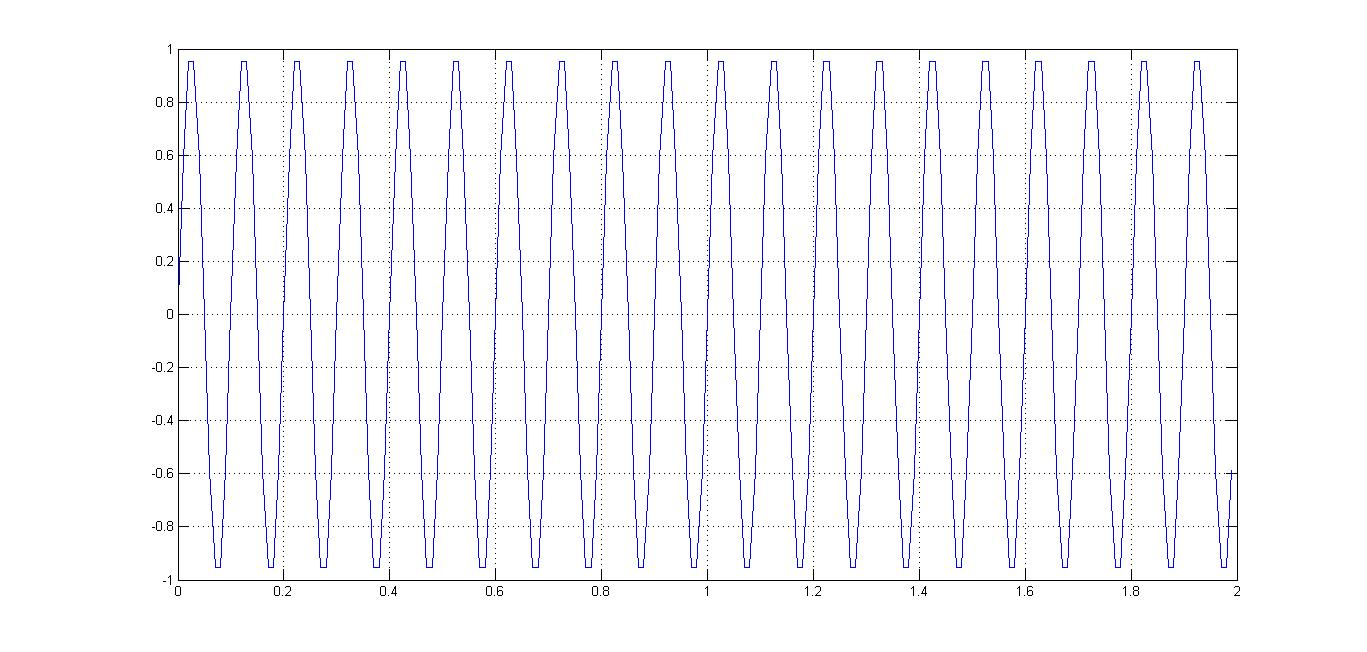
\includegraphics[angle=0, scale = 0.3]{sint.jpg}
рис. 1 Временная характеристика чистого синусоидального сигнала
\end{center}
\begin{center}
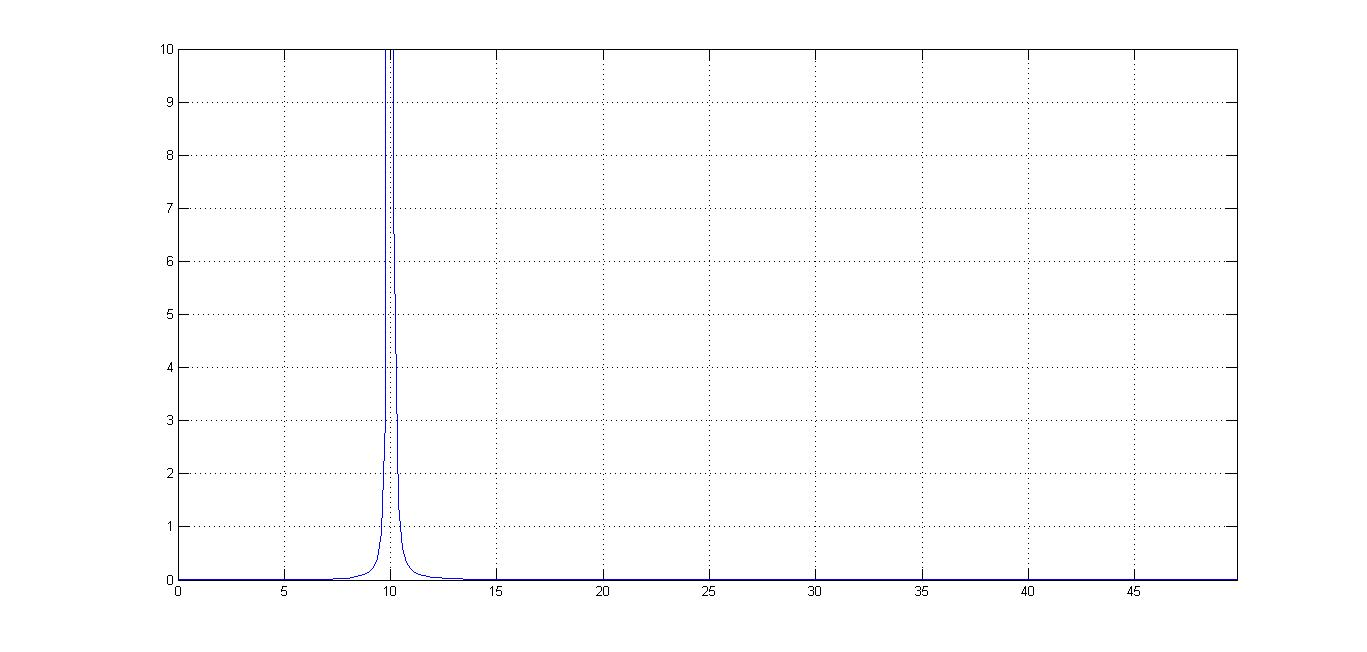
\includegraphics[angle=0, scale = 0.3]{sinch.jpg}
\end{center}
рис. 2. Частотная характеристика чистого синусоидального сигнала
\end{figure}
\begin{figure}
\begin{center}
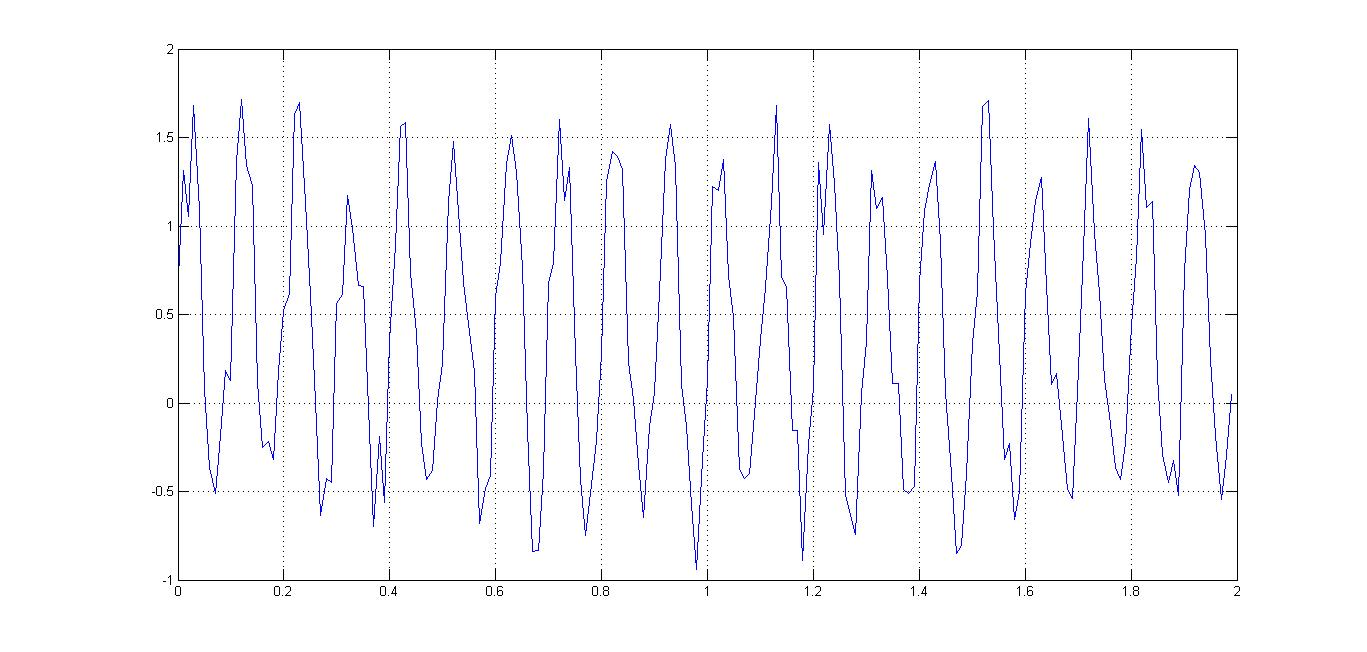
\includegraphics[angle=0, scale = 0.3]{nsint.jpg}
\end{center}
рис. 3. Временная характеристика зашумленного синусоидального сигнала
\begin{center}
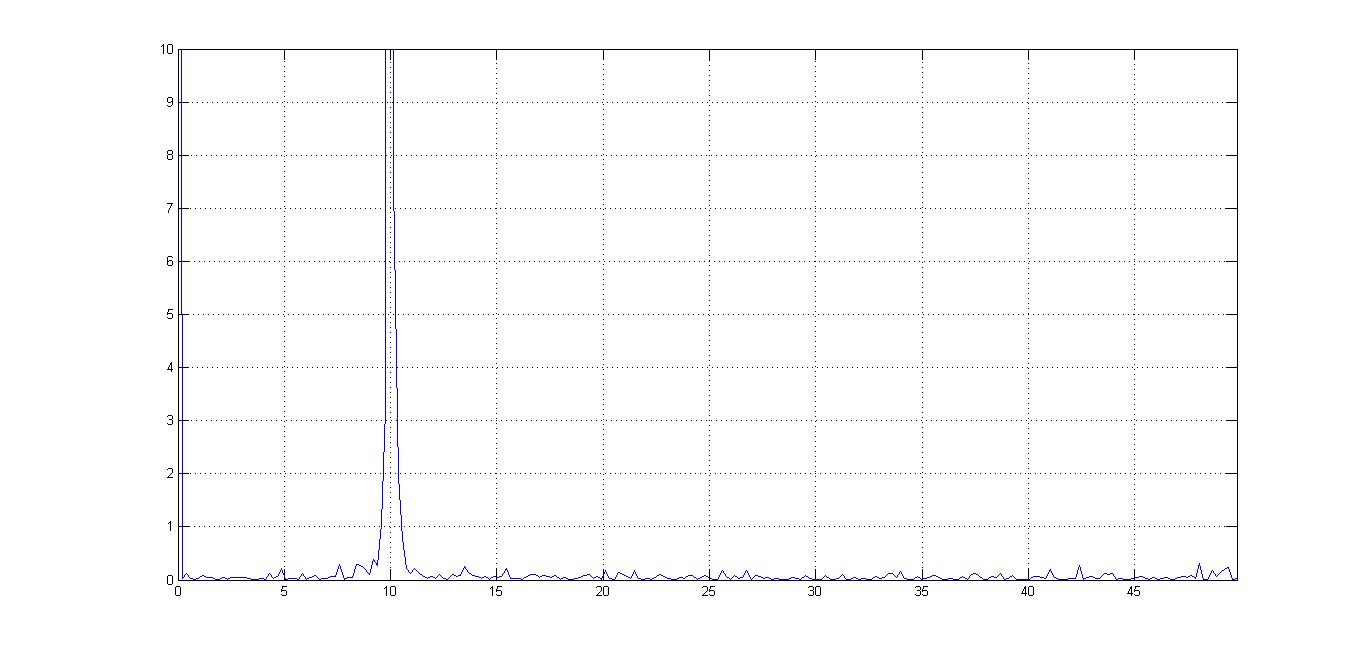
\includegraphics[angle=0, scale = 0.3]{nsinch.jpg}
\end{center}
рис. 4. Частотная характеристика зашумленного синусоидального сигнала
\end{figure}
Как видно из графиков, регулярная составляющая, как у чистого синусоидальног осигнала, так и у зашумленного равна 10Гц. Временная же характеристика чистого и зашумленного сигнала отличается достаточно сильно, хотя в обоих случаях заметны общие черты.
\chapter{Вывод}
В ходе лабораторной работы в среде MATLAB были промоделированны чистый и зашумленный синусоидальные сигналы с нулевыми начальными фазами, а так же были полученны их временные и частотные характеристики. Было выяснено, что при добавлении к чистому синусоидальному сигналу шумов, его регулярная составляющая остается прежней. Для выявления регулярной составляющей в данной работе использовалось одномерное прямое преобразование Фурье на основе 512 точек. Такое количество опорных точек было выбрано из соображений скорости рассчета и погрешности вычислений. Так как большее количество точек привело бы к заметному увеличению времени вычислений. Стоит так же отметить, что количество точек не случайно было выбрано кратным степени двойки ,т.к. такое соотношение обеспечивает максимальную скорость вычислений при использовании преобразования Фурье. Результаты вычислений являются достаточно точными, но тем не менее дают результат с определенной погрешностью. Это обусловленно двумя факторами:
\begin{itemize}
\item Дискретность представления сигнала
\item Конечность сигнала во времени
\end{itemize}
Из-за вышеперечисленных факторов мы не можем получить абсолютно точное значение, т.к. вычислительные ресурсы ограниченны, что в свою очередь накладывает ограничение на количество точек, участвующих в преобразовании Фурье, а так же мы не можем моделировать функцию бесконечно. Однако, мы получили приблизительный результат, который близок к теоретически ожидаемому. Однако, если бы мы использовали значительно меньшее количество точек, то результаты могли бы различаться очень значительно.
\end{document}
